% $Id: template.tex 11 2007-04-03 22:25:53Z jpeltier $

%\documentclass{vgtc}                          % final (conference style)
\documentclass[review]{vgtc}                 % review
%\documentclass[widereview]{vgtc}             % wide-spaced review
%\documentclass[preprint]{vgtc}               % preprint
%\documentclass[electronic]{vgtc}             % electronic version

%% Uncomment one of the lines above depending on where your paper is
%% in the conference process. ``review'' and ``widereview'' are for review
%% submission, ``preprint'' is for pre-publication, and the final version
%% doesn't use a specific qualifier. Further, ``electronic'' includes
%% hyperreferences for more convenient online viewing.

%% Please use one of the ``review'' options in combination with the
%% assigned online id (see below) ONLY if your paper uses a double blind
%% review process. Some conferences, like IEEE Vis and InfoVis, have NOT
%% in the past.

%% Figures should be in CMYK or Grey scale format, otherwise, colour 
%% shifting may occur during the printing process.

%% These three lines bring in essential packages: ``mathptmx'' for Type 1 
%% typefaces, ``graphicx'' for inclusion of EPS figures. and ``times''
%% for proper handling of the times font family.

\usepackage{mathptmx}
\usepackage{graphicx}
\usepackage{times}
\usepackage{mathtools}
\usepackage{cleveref}
\usepackage{textcomp}
\usepackage{gensymb}
\usepackage[detect-all]{siunitx}
%% We encourage the use of mathptmx for consistent usage of times font
%% throughout the proceedings. However, if you encounter conflicts
%% with other math-related packages, you may want to disable it.

%% If you are submitting a paper to a conference for review with a double
%% blind reviewing process, please replace the value ``0'' below with your
%% OnlineID. Otherwise, you may safely leave it at ``0''.
\onlineid{0}

%% declare the category of your paper, only shown in review mode
\vgtccategory{Research}

%% allow for this line if you want the electronic option to work properly
\vgtcinsertpkg

%% In preprint mode you may define your own headline.
%\preprinttext{To appear in an IEEE VGTC sponsored conference.}

%% Paper title.

\title{NvPipe: A Lightweight H264-based Hardware Accelerated Image Compression Library}

%% This is how authors are specified in the conference style

%% Author and Affiliation (single author).
%%\author{Roy G. Biv\thanks{e-mail: roy.g.biv@aol.com}}
%%\affiliation{\scriptsize Allied Widgets Research}

%% Author and Affiliation (multiple authors with single affiliations).
%%\author{Roy G. Biv\thanks{e-mail: roy.g.biv@aol.com} %
%%\and Ed Grimley\thanks{e-mail:ed.grimley@aol.com} %
%%\and Martha Stewart\thanks{e-mail:martha.stewart@marthastewart.com}}
%%\affiliation{\scriptsize Martha Stewart Enterprises \\ Microsoft Research}

%% Author and Affiliation (multiple authors with multiple affiliations)
%%\author{Roy G. Biv\thanks{e-mail: roy.g.biv@aol.com}\\ %
%%        \scriptsize Starbucks Research %
%%\and Ed Grimley\thanks{e-mail:ed.grimley@aol.com}\\ %
%%     \scriptsize Grimley Widgets, Inc. %
%%\and Martha Stewart\thanks{e-mail:martha.stewart@marthastewart.com}\\ %
%%     \parbox{1.4in}{\scriptsize \centering Martha Stewart Enterprises \\ Microsoft Research}}
\author{Jie Jiang \thanks{e-mail: jjiang24@uic.edu}\\ %
        \scriptsize University of Illinois at Chicago %
\and Thomas Fogal\thanks{e-mail: tfogal@nvidia.com}\\ %
     \scriptsize NVIDIA %
\and Cliff Woolley\thanks{e-mail: jwoolley@nvidia.com}\\ %
     \scriptsize NVIDIA %
\and Peter Messmer\thanks{e-mail: pmessmer@nvidia.com}\\ %
     \scriptsize NVIDIA} %


%% A teaser figure can be included as follows, but is not recommended since
%% the space is now taken up by a full width abstract.
%\teaser{
%  \includegraphics[width=1.5in]{sample.eps}
%  \caption{Lookit! Lookit!}
%}

%% Abstract section.
\abstract{
Hardware video encoding can lower the perceived latency for remote visualization. NvPipe is a lightweight library that simplifies the use of NVIDIA's video compression hardware. We achieve overall latencies below 15ms with compression ratios of approximately 0.7\%. To verify its applicability in real world scenarios, we integrated NvPipe into ParaView. NvPipe offloads the encoding within ParaView to the GPU and compresses images 30 times better as well. } % end of abstract

%% ACM Computing Classification System (CCS). 
%% See <http://www.acm.org/class/1998/> for details.
%% The ``\CCScat'' command takes four arguments.

%\CCScatlist{ 
%  \CCScat{K.6.1}{Management of Computing and Information Systems}%
%{Project and People Management}{Life Cycle};
%  \CCScat{K.7.m}{The Computing Profession}{Miscellaneous}{Ethics}
%}

%% Copyright space is enabled by default as required by guidelines.
%% It is disabled by the 'review' option or via the following command:
% \nocopyrightspace

%%%%%%%%%%%%%%%%%%%%%%%%%%%%%%%%%%%%%%%%%%%%%%%%%%%%%%%%%%%%%%%%
%%%%%%%%%%%%%%%%%%%%%% START OF THE PAPER %%%%%%%%%%%%%%%%%%%%%%
%%%%%%%%%%%%%%%%%%%%%%%%%%%%%%%%%%%%%%%%%%%%%%%%%%%%%%%%%%%%%%%%%

\begin{document}

%% The ``\maketitle'' command must be the first command after the
%% ``\begin{document}'' command. It prepares and prints the title block.

%% the only exception to this rule is the \firstsection command
\firstsection{Introduction}

\maketitle

Image compression is commonly used in distributed visualization systems to overcome limitations of available bandwidth. Conventional image compression approach focuses on removing redundant information within each image without necessarily utilizing the inter-frame coherency.

H.264 is a block-oriented motion-compensation-based video compression standard \cite{wiegand2003overview}. It provides high compression capability at the cost of significant computational expenses. NVIDIA provides hardware accelerated H.264 encoder since Kepler archetecture. It enables real-time encoding with minimum overhead and it has been integrated into multimedia framework FFmpeg \cite{ffmpeg}. 

\section{Implementation}

NvPipe is built on top of FFmpeg to provide compatibility across systems with or without hardware accelerated H264 compression. Although NvPipe accepts images with format RGB/RGBA/YUV, it will convert the image into NV12 to before passing it to FFmpeg/NVENC. As is the decompressed image.

\subsection{Design}

NvPipe could use both hardware accelerated NVIDIA codec and libx264 codec. Using widely applicable default values requires little effort to integrate into existing systems. The library simplifies exposed interfaces by providing generic default configuration. For example the default group of pictures (GOP) size is 60 and I:P frame ratio is 1:59.

Compression and decompression with NvPipe is implemented in a synchronous manner without frame latency. Each input frame/packet will return an output packet/frame. NvPipe handles only image compression/decompression. It leaves memory allocation and streaming to user for ease of integration.

\subsection{Performance}

The performance of the compression library is measured by 3 factors: computational efficiency, compression ratio and image quality preservation.

\subsubsection{Compression Ratio}

%put the reference here: http://www.adobe.com/content/dam/Adobe/en/devnet/video/articles/h264_primer/h264_primer.pdf
Compression ratio is determined by the average bitrate parameter of NvPipe. A guideline for bitrate setting is through Kush Gauge \cite{iszaidyinvestigation}:

\begin{equation}
\label{eq:bitrate}
 bitrate = resolution * \text{ fps} * f_m * 0.07
\end{equation}

Where \(f_m\) is the motion factor that defines the estimated motion of the video with value \numrange{1}{4}. While 1 indicates lowest motion and 4 the highest. NvPipe default bitrate uses \cref{eq:bitrate} with \(f_m=4\).

Assuming we are given 8bit RGB image. Each pixel contains 3 channels. The compression ratio could be calculated by dividing bitrate to total image size per second.

\begin{equation}
\label{eq:compress_ratio}
 r = \frac{ \text{ bitrate}}{ \text{ resolution} * \text{fps} * 3 * 8} = 0.07f_m/3/8 = 0.29f_m\%
\end{equation}

\subsubsection{Image Quality}

NvPipe could introduce artifacts during conversion and compression stage. Format conversion from RGB to YUV applies chroma subsampling which introduces artifacts on sharp edges. And NvPipe H.264 compression is configured as high performance low latency mode that is not lossless. \cref{fig:quality} shows that very fine features are decently preserved through NvPipe.

\begin{figure}[h]
  \centering
  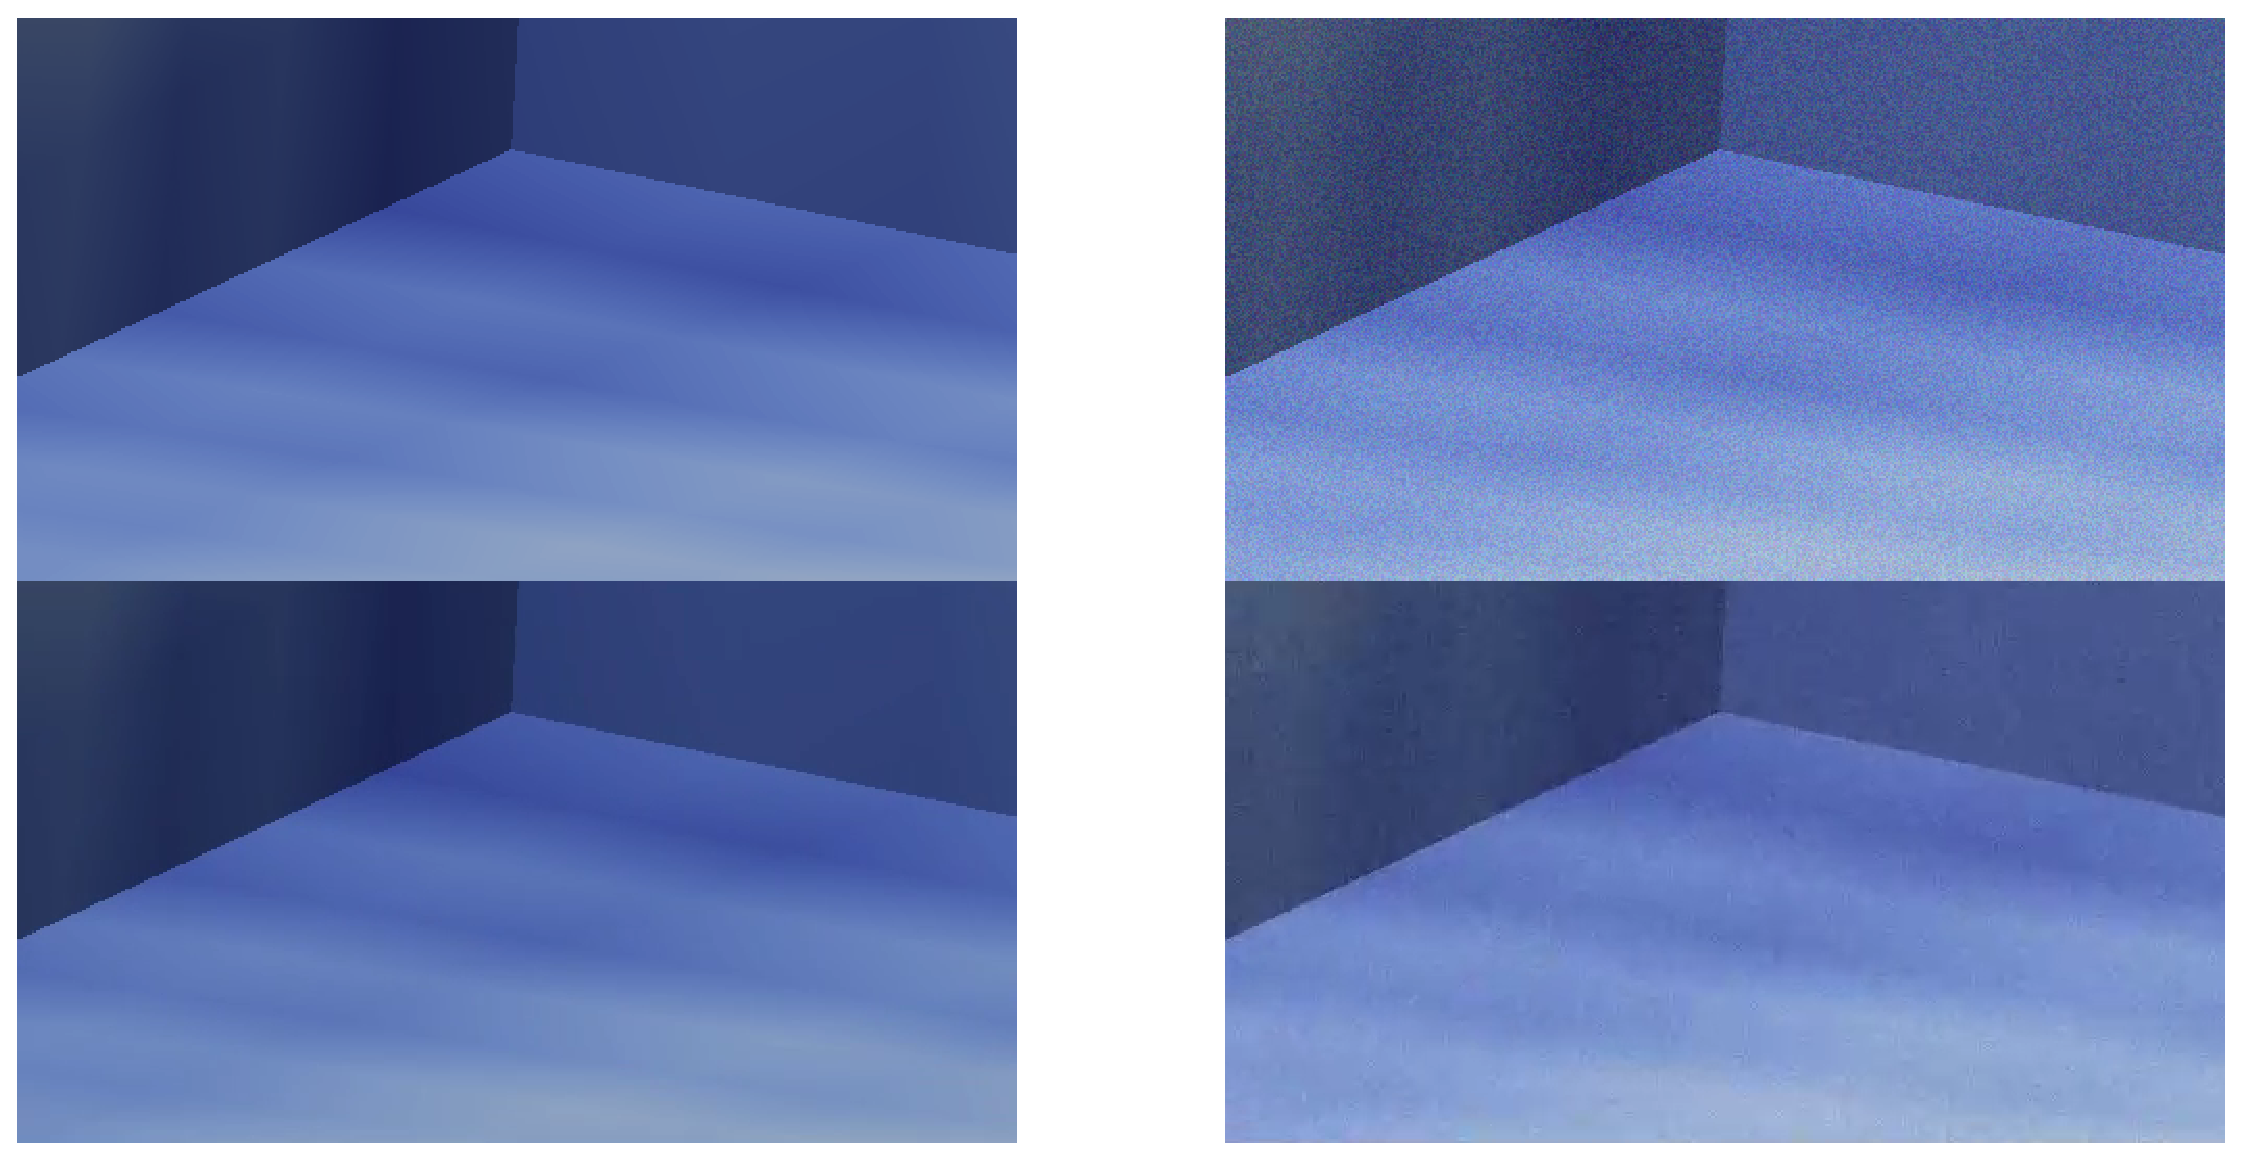
\includegraphics[width=\columnwidth]{quality.eps}
  \caption{1080P image rendered from randomly rotating volume data and compressed using bitrate with \(f_m=4\). Average stractural similarity (SSIM) between the images are 98\% \cite{wang2004image}. Looking at a the block of 60x60 pixels. The left block is the original image while the right block is the recovered image, we can see fine features has been well preserved. }
  \label{fig:quality}
\end{figure}

\section{Results}

%Our experiment setup contains two parts. In part one we benchmark the performance of our library given different resolutions and bitrates. In part two we implement vtkNvpipeCompressor to integrate NvPipe into Paraview. We create a distribute visualization use case and compared the performance of NvPipe with ParaView's native built-in compressor.
Our experiment runs on a Linux machine powered by NVIDIA GeForce GTX 1080 (PASCAL) graphics card.

We first run the benchmark of NvPipe on RGB images. We set up experiment groups using 4 common resolutions. For each one we run 3 cases with low bitrate, medium bitrate and high bitrate settings. The medium setting uses \cref{eq:bitrate} with \(f_m = 1\) to calculate the bitrate. While low and high uses \(f_m\) of 0.5 and 2 respectively. Each case runs 300 cycles of compressing and decompressing of consecutive images generated with moving color pattern.

The second part we integrate NvPipe into ParaView and compare the performance of NvPipe with and without hardware acceleration to built-in compressors utilizing lz4, squirt and Zlib. NvPipe uses high bitrate setting with \(f_m=4\) for best image quality. For configuration of ParaView compressors: Lz4 uses quality level 0. Squirt uses compression level 5. Zlib uses compression level of 9 for slow compression with highest compression ratio, color space reduction level of 5 and alpha channel stripping. Zlib fast uses compression level of 1 for fast compression with lowest compression ratio while other parameters remain the same. The experiments use 300 cycles of 1080P RGBA images of rotating volume data. One case uses fixed small rotation angle of \(1.2\degree\) per frame. And the other uses large rotation angle of \(40\degree\) per frame.

\subsection{NvPipe Benchmark}
% library benchmark

The benchmark experiment shows linear scalability of NvPipe to image size. Given the total number of million pixels of the image to be \(n_p\) and motion factor used for bitrate calculation to be \(f_m\). Linear regression analysis of compression time \(t_c\) and decompression time \(t_d\) generates the following models: \(t_c=2.27n_p+0.16f_m+0.86\) and \(t_d=1.60n_p+0.02f_m+0.89\) with \(R^2_c=99.92\%\) and \(R^2_d=99.97\%\). Performance is linear to total number of pixels in the image with trivial influence from the bitrate multipliccation factor used.
%%%%%%%%%%%%%%%%%%%%%%%%%%%%%%%%%
%   discuss it if extra room appears later.
%
%Each image compression or decompression call to NvPipe consists of format conversion and encoding or decoding API calls. Computational complexity for both tasks are linear to the totally number of pixels of the input or output image. So we could expect the overall complexity of our compression and decompression call remains linear to the image size.

\cref{tab:experiment_setup} lists general bandwidth requirements and performance for common resolution. 

\begin{table}[h]
  \caption{Computational scalability benchmark measuring average compression and decompression time per frame during 300 frames of RGB images with moving pattern}
  \label{tab:experiment_setup}
  \scriptsize
  \begin{center}
    \begin{tabular}{cccc}
      Resolution & Bitrate(mbps) & Compress(ms) & Decompress(ms)\\
    \hline
      1024x768 & 1.651 & 2.8057 & 2.1170\\
      1280x720 & 1.935 & 3.4793 & 2.4304\\
      1920x1080 & 4.355 & 5.4358 & 4.2876\\
      4096x2160 & 18.579 & 21.2504 & 15.0976
    \end{tabular}
  \end{center}
\end{table}

\subsection{ParaView Integration}

\begin{figure}[htb]
  \centering
  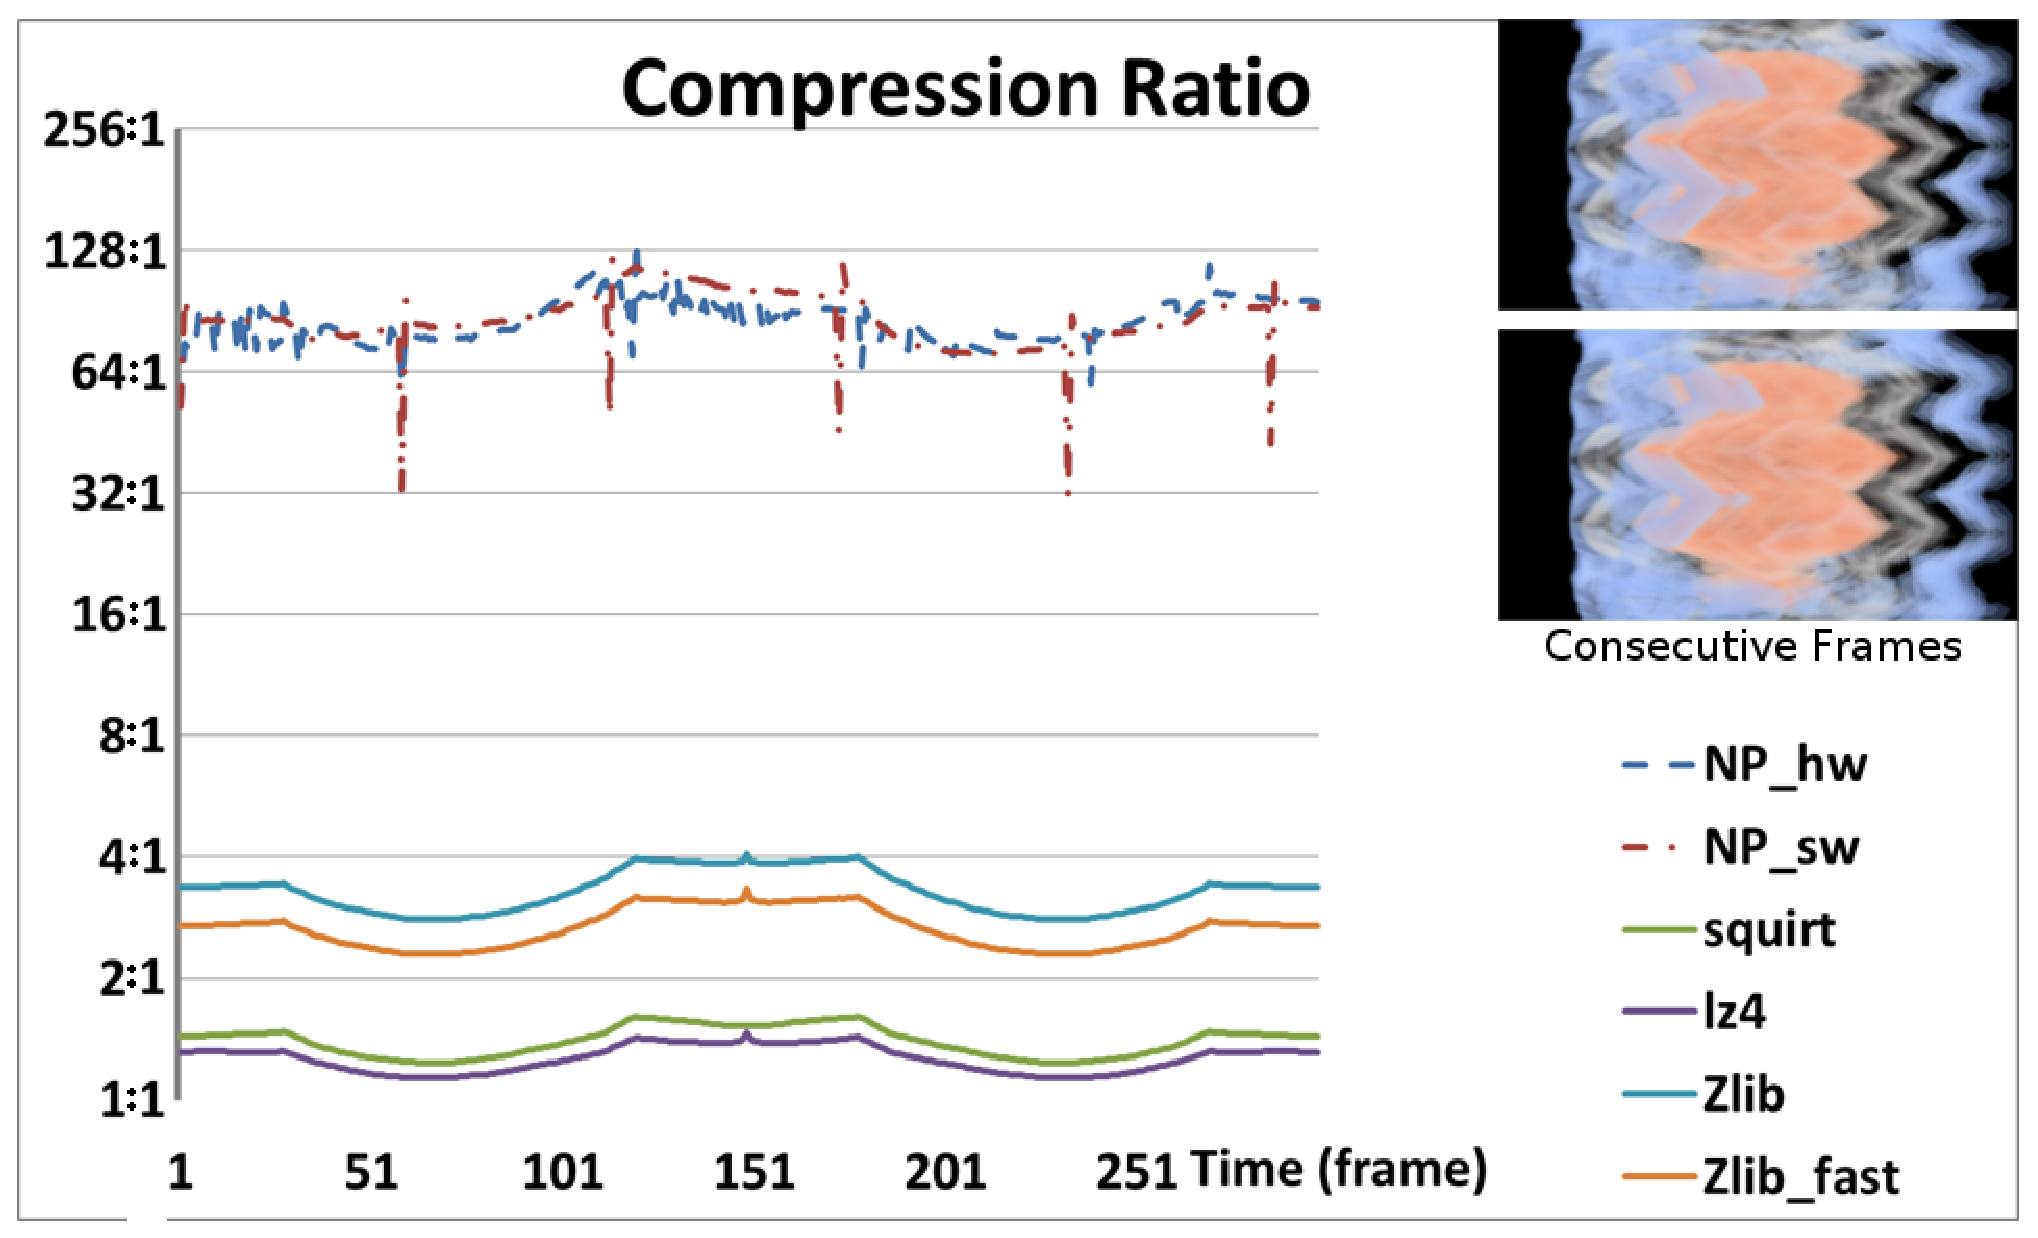
\includegraphics[width=\columnwidth]{compressRatio.eps}
  \caption{Compression ratio during small rotation experiemnt: i. NvPipe compressor has a huge compression ratio advantage of below 1\% versus ParaView compressors staying between 25\% to 90\%. ii. ParaView compressors are highly sensitive to data, notice the symmetric pattern due to the \(360\degree\) rotation, while NvPipe compression ratio stays stable except for the peak due to the key frame every 60 frames. }
  \label{fig:compressRatio}
\end{figure}
  %ParaView built-in compressors use the primary axis on the left while NvPipe hardware and software compressors use the secondary axis on the right. 

Distributed ParaView server uses NvPipe to compress RGBA image buffer and streams compressed image to display client. Our experiment launches both server and client on the same machine to eliminate network latency.

\cref{fig:compressRatio} shows the compression ratio over time of a slowly rotating volume data. It exhibits the image compression ratio benefit and stability of NvPipe over built-in compressors in ParaView under normal interactive visualization.

% discuss the bandwidth reduction ( compare other paraview compressor )
For more generic case, our experiments runs 5 sets of 300 frames of randomly rotating volume data at resolution of 1080P.
The efficiency in \cref{fig:time} shows that although software-based NvPipe suffers from slow compression, the hardware accelerated NvPipe compressor outperforms other tested compressor in both encoding and decoding time.

The compression ratio on the first 2 rows in \cref{tab:latency}. NvPipe has 43 times better compression ratio comparing to fast Zlib, which is the best compressor tested in Paraview.
The theoretical aggregated latency could be calculated through \cref{eq:latency}, where communication time \(t_{network}={compressed\, image\, size}/{BW}\). 

\begin{equation}
\label{eq:latency}
T_{latency}=t_{compression}+t_{decompression}+t_{network}
\end{equation}

Assume we have 100mbps available bandwidth, for each compressor image size \(s_i=1920*1080*8*3*{ratio}\) we could calculate the communication time for each compressor. Combining data from \cref{fig:time} we get the overall latency in \cref{tab:latency}.

% discuss encoding/decoding time --> framerate / latency 
\begin{figure}[t]
  \centering
  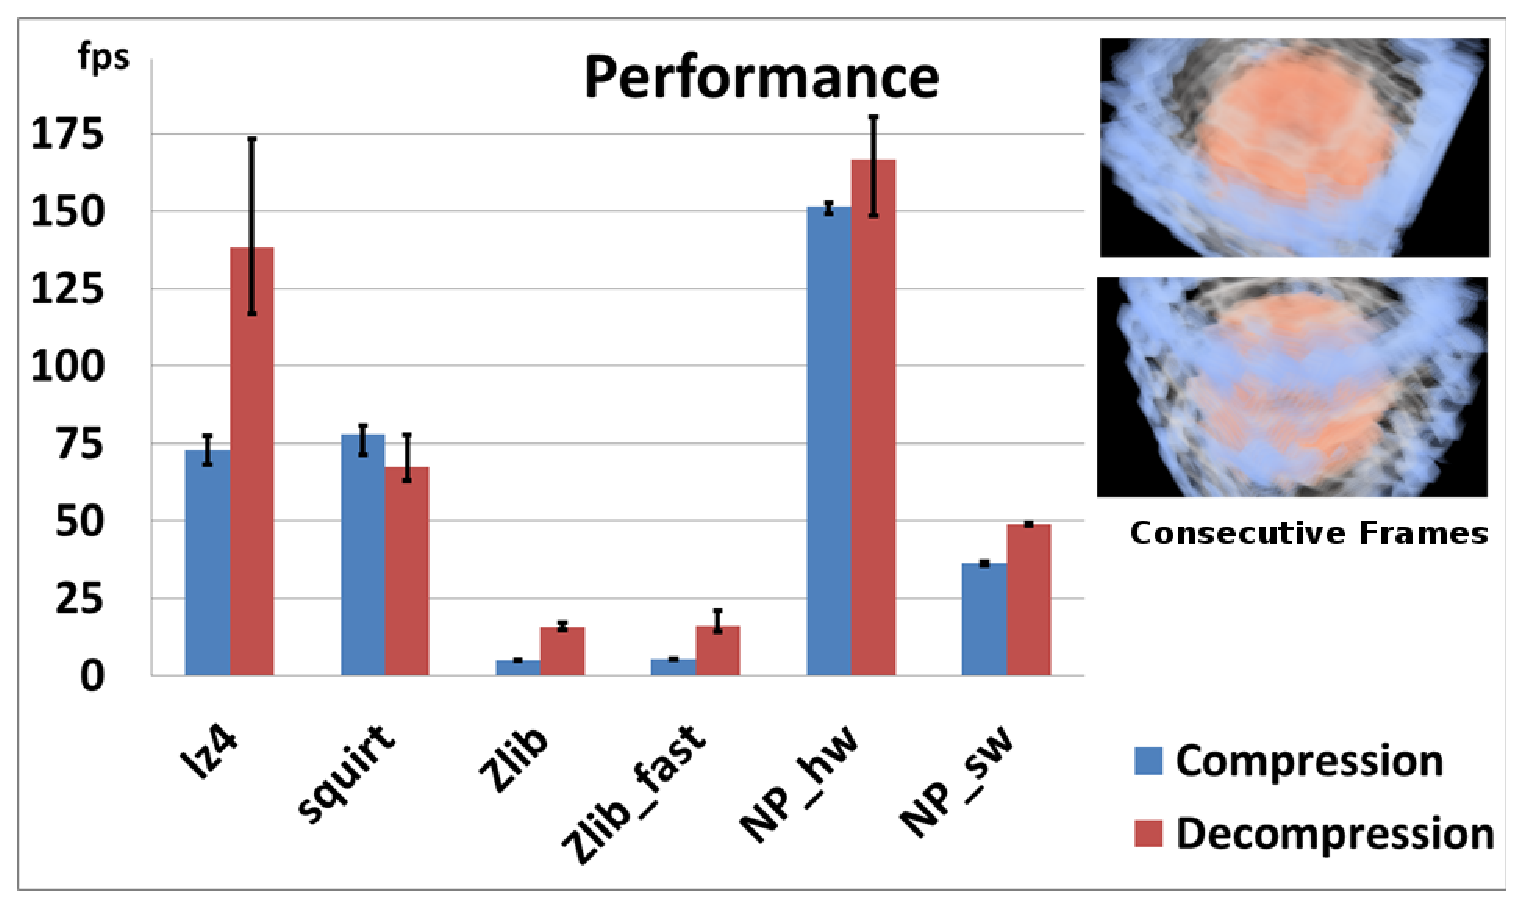
\includegraphics[width=\columnwidth]{Performance.eps}
  \caption{ Average compress and decompress time of large rotation experiment. For NvPipe we stack the time of format conversion and compress/decompress time. NvPipe software approach takes much longer time for image compression. While NvPipe hardware compressor outperforms other compressors.}
  \label{fig:time}
\end{figure}

\begin{table}[htb]
  \caption{Average compression ratio and theoretical latency of large rotation experiment. The lower ratio means better compressed. H.264 has much better compression ratio as well as higher computational complexity as can be seen from the encoding time of NvPipe software. For the overall latency NvPipe hardware approach has 4 times speed up comparing to the second fasted compressor LZ4}
  \label{tab:latency}
  \scriptsize
  \begin{center}
    \begin{tabular}{ccccccc}
      & LZ4 & Squirt & Zlib & Zlib\_fast & NP\_hw & NP\_sw \\
    \hline
      ratio(\%) & 79.4 & 69.8 & 30.7 & 30.4 & 0.70 & 0.65 \\
      std dev & 0.061 & 0.061 & 0.033 & 0.034 & 0.001 & 0.001\\
      comm(ms) & 39.49 & 34.71 & 15.15 & 15.28 & 0.35 & 0.32 \\
      Latency(ms) & 57.23 & 50.22 & 119.45 & 128.02 & 13.14 & 76.26
    \end{tabular}
  \end{center}
\end{table}


\section{Conclusion}

%NvPipe exhibits competitive efficiency among other compressors in \cref{fig:time}. The average overall compression and decompression time is only 12.78ms. And the average encoding and decoding time for FFmpeg API call are 3.938ms and 3.029ms. They yield framerates of 254fps and 330fps respectively. Because of the overhead introduced through FFmpeg wrapper they are expected to be lower than 398fps/658fps released by \cite{ref_1}.% cite nv codec menu.

NvPipe demonstrates great potential with its image quality preservation, compression ratio and efficiency. It could reduce overall latency and improve framerate for distributed visualization system with limited bandwidth. In future research it will be intereting to investigate the performance of lossless H.264 configuration and HEVC standard provided with NVIDIA codec 7.0 API.

%\acknowledgements{
%NVIDIA standard acknowledgement for funding?
%}

\pagebreak

\bibliographystyle{abbrv}
%%use following if all content of bibtex file should be shown
\nocite{*}
\bibliography{template}
\end{document}
